\documentclass[12pt,a4]{article}
\usepackage{physics, amsmath,amsfonts,amsthm,amssymb, mathtools,steinmetz, gensymb, siunitx}	% LOADS USEFUL MATH STUFF
\usepackage{xcolor,graphicx}
\usepackage{caption}
\usepackage{subcaption}
\usepackage[left=45pt, top=20pt, right=45pt, bottom=45pt ,a4paper]{geometry} 				% ADJUSTS PAGE
\usepackage{setspace}
\usepackage{tikz}
\usepackage{pgf,tikz,pgfplots,wrapfig}
\usepackage{mathrsfs}
\usepackage{fancyhdr}
\usepackage{float}
\usepackage{array}
\usepackage{booktabs,multirow}
\usepackage{bm}
\usepackage{tensor}
\usepackage{listings}
 \lstset{
    basicstyle=\ttfamily\small,
    numberstyle=\footnotesize,
    numbers=left,
    backgroundcolor=\color{gray!10},
    frame=single,
    tabsize=2,
    rulecolor=\color{black!30},
    title=\lstname,
    escapeinside={\%*}{*)},
    breaklines=true,
    breakatwhitespace=true,
    framextopmargin=2pt,
    framexbottommargin=2pt,
    inputencoding=utf8,
    extendedchars=true,
    literate={á}{{$\rho$}}1 {ã}{{\~a}}1 {é}{{\'e}}1,
}
\DeclareMathOperator{\sign}{sgn}
\DeclareMathOperator{\Div}{div}
\newcommand{\e}{\mathrm{d}}

\usetikzlibrary{decorations.text, calc}
\pgfplotsset{compat=1.7}

\usetikzlibrary{decorations.pathreplacing,decorations.markings}
\usepgfplotslibrary{fillbetween}

\newcommand{\vect}[1]{\boldsymbol{#1}}

\usepackage{hyperref}

%\usepackage[style= ACM-Reference-Format, maxbibnames=6, minnames=1,maxnames = 1]{biblatex}
%\addbibresource{references.bib}


\hypersetup{pdfborder={0 0 0},colorlinks=true,linkcolor=black,urlcolor=cyan,}
\allowdisplaybreaks

\title{
  \textsc{Quantum Information Homework 1}
}
  \author{\textsc{J L Gouws}
}

\date{\today
\\[1cm]}

\usepackage{graphicx}
\usepackage{array}


\begin{document}
\thispagestyle{empty}

\maketitle

Acknowledgements:
I received some unhelpful help from Pierre-Antoine Graham on the POVM question, and subsequently I received a lot of very appreciated help from Eirini.
\begin{enumerate}
  \item
    \begin{enumerate}
      \item
        For the state:
        \begin{equation*}
          |\Phi_{AB}^{+}\rangle = \frac{1}{\sqrt{2}}(| 00 \rangle + | 11 \rangle)
        \end{equation*}
        The density matrix is:
        \begin{align*}
          \rho &= |\Phi_{AB}^{+}\rangle\langle\Phi_{AB}^{+}|\\
               &= \frac{1}{2}(| 00 \rangle + | 11 \rangle)(\langle 00 | + \langle 11 |)\\
               &= \frac{1}{2}(| 00 \rangle \langle 00 | + | 11 \rangle \langle 00 | + | 00 \rangle \langle 11 | + | 11 \rangle \langle 11 |)
        \end{align*}
        And as a matrix:
        \begin{align*}
          \rho = 
            \frac{1}{2}
          \left(
          \begin{matrix}
            1 & 0 & 0 & 1\\
            0 & 0 & 0 & 0\\
            0 & 0 & 0 & 0\\
            1 & 0 & 0 & 1
          \end{matrix}
          \right)
        \end{align*}
        Which has one non-zero eigenvalue $1$ corresponding to the normalized eigenvector:
        \begin{align*}
             v = 
            \frac{1}{\sqrt{2}}
              \left(
              \begin{matrix}
                1 \\
                0 \\
                0 \\
                1 
              \end{matrix}
          \right)
        \end{align*}
        And hence the square root of the density matrix is:
        \begin{align*}
          \sqrt{\rho} 
            &= 
            \sqrt{1} v v^T \\
            &= 
            \frac{1}{2}
          \left(
          \begin{matrix}
            1 & 0 & 0 & 1\\
            0 & 0 & 0 & 0\\
            0 & 0 & 0 & 0\\
            1 & 0 & 0 & 1
          \end{matrix}
          \right)
        \end{align*}
        And:
        \begin{equation*}
          \sigma_y \otimes \sigma_y
          =
          \left(
          \begin{matrix}
            0
            \left[
            \begin{matrix}
              0 &-i\\
              i & 0
            \end{matrix}
            \right]
            &
            -i 
            \left[
            \begin{matrix}
              0 &-i\\
              i & 0
            \end{matrix}
            \right] \\
            i
            \left[
            \begin{matrix}
              0 &-i\\
              i & 0
            \end{matrix}
            \right]
            &
            0 
            \left[
            \begin{matrix}
              0 &-i\\
              i & 0
            \end{matrix}
            \right]
          \end{matrix}
          \right)
          =
          \left(
            \begin{matrix}
              0 & 0 & 0 & -1\\
              0 & 0 & 1 &  0\\
              0 & 1 & 0 &  0\\
             -1 & 0 & 0 &  0\\
            \end{matrix}
          \right)
        \end{equation*}
        And therefore:
        \begin{align*}
          \tilde\rho
            &= 
            \frac{1}{2}
            \left(
              \begin{matrix}
                0 & 0 & 0 & -1\\
                0 & 0 & 1 &  0\\
                0 & 1 & 0 &  0\\
               -1 & 0 & 0 &  0\\
              \end{matrix}
            \right)
            \left(
            \begin{matrix}
              1 & 0 & 0 & 1\\
              0 & 0 & 0 & 0\\
              0 & 0 & 0 & 0\\
              1 & 0 & 0 & 1
            \end{matrix}
            \right)
            \left(
              \begin{matrix}
                0 & 0 & 0 & -1\\
                0 & 0 & 1 &  0\\
                0 & 1 & 0 &  0\\
               -1 & 0 & 0 &  0\\
              \end{matrix}
            \right)
            \\
            &=
            \frac{1}{2}
            \left(
            \begin{matrix}
              1 & 0 & 0 & 1\\
              0 & 0 & 0 & 0\\
              0 & 0 & 0 & 0\\
              1 & 0 & 0 & 1
            \end{matrix}
            \right)\\
            &= \rho
        \end{align*}
        \begin{align*}
          \sqrt{\rho} \tilde\rho \sqrt{\rho} 
            &= 
            \frac{1}{8}
            \left(
            \begin{matrix}
              1 & 0 & 0 & 1\\
              0 & 0 & 0 & 0\\
              0 & 0 & 0 & 0\\
              1 & 0 & 0 & 1
            \end{matrix}
            \right)
            \left(
            \begin{matrix}
              1 & 0 & 0 & 1\\
              0 & 0 & 0 & 0\\
              0 & 0 & 0 & 0\\
              1 & 0 & 0 & 1
            \end{matrix}
            \right)
            \left(
            \begin{matrix}
              1 & 0 & 0 & 1\\
              0 & 0 & 0 & 0\\
              0 & 0 & 0 & 0\\
              1 & 0 & 0 & 1
            \end{matrix}
            \right)
            \\
            &=
            \frac{1}{2}
            \left(
            \begin{matrix}
              1 & 0 & 0 & 1\\
              0 & 0 & 0 & 0\\
              0 & 0 & 0 & 0\\
              1 & 0 & 0 & 1
            \end{matrix}
            \right)\\
            &= \rho
        \end{align*}
        And the square root of this matrix is just:
        \begin{align*}
          R = 
          \sqrt{\rho}
          &= 
            \frac{1}{2}
            \left(
            \begin{matrix}
              1 & 0 & 0 & 1\\
              0 & 0 & 0 & 0\\
              0 & 0 & 0 & 0\\
              1 & 0 & 0 & 1
            \end{matrix}
            \right)
        \end{align*}
        This matrix has one non-zero eigenvalue which is one and so:
        \begin{equation*}
          C[\rho] = 1
        \end{equation*}
        For the state:
        \begin{equation*}
          |\psi_{AB}\rangle = | 00 \rangle
        \end{equation*}
        And:
        \begin{equation*}
          \rho_\psi = 
            \left(
            \begin{matrix}
              1 & 0 & 0 & 0\\
              0 & 0 & 0 & 0\\
              0 & 0 & 0 & 0\\
              0 & 0 & 0 & 0
            \end{matrix}
            \right)
        \end{equation*}
        Clearly:
        \begin{equation*}
          \sqrt{\rho_\psi} = 
            \left(
            \begin{matrix}
              1 & 0 & 0 & 0\\
              0 & 0 & 0 & 0\\
              0 & 0 & 0 & 0\\
              0 & 0 & 0 & 0
            \end{matrix}
            \right)
        \end{equation*}
        And:
        \begin{align*}
          \tilde\rho_\psi
            &= 
            \left(
              \begin{matrix}
                0 & 0 & 0 & -1\\
                0 & 0 & 1 &  0\\
                0 & 1 & 0 &  0\\
               -1 & 0 & 0 &  0\\
              \end{matrix}
            \right)
            \left(
            \begin{matrix}
              1 & 0 & 0 & 0\\
              0 & 0 & 0 & 0\\
              0 & 0 & 0 & 0\\
              0 & 0 & 0 & 0
            \end{matrix}
            \right)
            \left(
              \begin{matrix}
                0 & 0 & 0 & -1\\
                0 & 0 & 1 &  0\\
                0 & 1 & 0 &  0\\
               -1 & 0 & 0 &  0\\
              \end{matrix}
            \right)
            \\
            &=
            \left(
            \begin{matrix}
              0 & 0 & 0 & 0\\
              0 & 0 & 0 & 0\\
              0 & 0 & 0 & 0\\
              0 & 0 & 0 & 1
            \end{matrix}
            \right)
        \end{align*}
        Now:
        \begin{equation*}
          \sqrt{\rho_\psi} \tilde\rho_\psi \sqrt{\rho_\psi} =
            \left(
            \begin{matrix}
              1 & 0 & 0 & 0\\
              0 & 0 & 0 & 0\\
              0 & 0 & 0 & 0\\
              0 & 0 & 0 & 0
            \end{matrix}
            \right)
            \left(
            \begin{matrix}
              0 & 0 & 0 & 0\\
              0 & 0 & 0 & 0\\
              0 & 0 & 0 & 0\\
              0 & 0 & 0 & 1
            \end{matrix}
            \right)
            \left(
            \begin{matrix}
              1 & 0 & 0 & 0\\
              0 & 0 & 0 & 0\\
              0 & 0 & 0 & 0\\
              0 & 0 & 0 & 0
            \end{matrix}
            \right)
            =
            \left(
            \begin{matrix}
              0 & 0 & 0 & 0\\
              0 & 0 & 0 & 0\\
              0 & 0 & 0 & 0\\
              0 & 0 & 0 & 0
            \end{matrix}
            \right)
        \end{equation*}
        Which has all zero eigenvalues and hence $C[\rho_\psi] = 0$.
      \item
        For the Bell state:
        \begin{equation*}
          \rho_{AB} = \frac{1}{\sqrt{2}}(\left| 0\right\rangle_A\left| 0\right\rangle_B\left\langle 0\right|_A\left\langle 0\right|_B + \left| 1\right\rangle_A\left| 1\right\rangle_B\left\langle 0\right|_A\left\langle 0\right|_B + \left| 0\right\rangle_A\left| 0\right\rangle_B\left\langle 1\right|_A\left\langle 1\right|_B + \left| 1\right\rangle_A\left| 1\right\rangle_B\left\langle 1\right|_A\left\langle 1\right|_B)
        \end{equation*}
        And hence:
        \begin{equation*}
          \rho_{AB}^\Gamma = \frac{1}{2}(\left| 0\right\rangle_A\left| 0\right\rangle_B\left\langle 0\right|_A\left\langle 0\right|_B + \left| 1\right\rangle_A\left| 0\right\rangle_B\left\langle 0\right|_A\left\langle 1\right|_B + \left| 0\right\rangle_A\left| 1\right\rangle_B\left\langle 1\right|_A\left\langle 0\right|_B + \left| 1\right\rangle_A\left| 1\right\rangle_B\left\langle 1\right|_A\left\langle 1\right|_B)
        \end{equation*}
        Or as a matrix:
        \begin{equation*}
          \rho_{AB}^\Gamma = \frac{1}{2}
          \left(
            \begin{matrix}
              1 & 0 & 0 & 0\\
              0 & 0 & 1 & 0\\
              0 & 1 & 0 & 0\\
              0 & 0 & 0 & 1
            \end{matrix}
          \right)
        \end{equation*}

        Now:
        \begin{align*}
          ||\rho^\Gamma || 
            &= \tr \sqrt{
              \frac{1}{4}
            \left(
              \begin{matrix}
                1 & 0 & 0 & 0\\
                0 & 0 & 1 & 0\\
                0 & 1 & 0 & 0\\
                0 & 0 & 0 & 1
              \end{matrix}
            \right)
            \left(
              \begin{matrix}
                1 & 0 & 0 & 0\\
                0 & 0 & 1 & 0\\
                0 & 1 & 0 & 0\\
                0 & 0 & 0 & 1
              \end{matrix}
            \right)
          }\\
          &= \frac{1}{2}\tr \sqrt{
            \left(
              \begin{matrix}
                1 & 0 & 0 & 0\\
                0 & 1 & 0 & 0\\
                0 & 0 & 1 & 0\\
                0 & 0 & 0 & 1
              \end{matrix}
            \right)
          }\\
          & = 2
        \end{align*}
        Hence the negativity is:
        \begin{equation*}
          \mathcal{N} [\rho] = \frac{2 - 1}{2} =\frac{1}{2} 
        \end{equation*}

        Take the state $| 00 \rangle$ its density matrix is:
        \begin{equation*}
          \rho = | 0 \rangle |0 \rangle \langle 0 | \langle 0 | \Rightarrow \rho^\Gamma = | 0 \rangle |0 \rangle \langle 0 | \langle 0 |
        \end{equation*}
        Now:
        \begin{align*}
          ||\rho^\Gamma || &= \tr \sqrt{
            \left(
              \begin{matrix}
                1 & 0 & 0 & 0\\
                0 & 0 & 0 & 0\\
                0 & 0 & 0 & 0\\
                0 & 0 & 0 & 0
              \end{matrix}
            \right)
            \left(
              \begin{matrix}
                1 & 0 & 0 & 0\\
                0 & 0 & 0 & 0\\
                0 & 0 & 0 & 0\\
                0 & 0 & 0 & 0
              \end{matrix}
            \right)
          }\\
          &= \tr \sqrt{
            \left(
              \begin{matrix}
                1 & 0 & 0 & 0\\
                0 & 0 & 0 & 0\\
                0 & 0 & 0 & 0\\
                0 & 0 & 0 & 0
              \end{matrix}
            \right)
          }\\
          & = 1
        \end{align*}
        And therefore:
        \begin{equation*}
          \mathcal{N} [\rho] = \frac{||\rho^\Gamma||_1 - 1}{2} = 0
        \end{equation*}
      \item
        The density matrix here is:
        \begin{align*}
          \rho_{AB} &= \frac{1}{4} (| 0 \rangle_A \langle 0| + | 1 \rangle_A \langle 1|) \otimes (| 0 \rangle_B \langle 0| + | 1 \rangle_B \langle 1|)\\
                    &= \frac{1}{4} (| 0  0 \rangle \langle 0 0| + | 1 0 \rangle \langle 1 0 | + | 0 1 \rangle \langle 0 1 | + | 1 1 \rangle \langle 1 1|)\\
                    &= \frac{1}{4} 
                    \left(
                     \begin{matrix}
                       1 & 0 & 0 & 0\\
                       0 & 1 & 0 & 0\\
                       0 & 0 & 1 & 0\\
                       0 & 0 & 0 & 1
                     \end{matrix}
                    \right)
        \end{align*}
        And
        \begin{align*}
          \rho^\Gamma 
                    &= \frac{1}{4} (| 0 \rangle_A \langle 0| + | 1 \rangle_A \langle 1|) \otimes (| 0 \rangle_B \langle 0| + | 1 \rangle_B \langle 1|)\\
                    &= \frac{1}{4} (| 0  0 \rangle \langle 0 0| + | 1 0 \rangle \langle 1 0 | + | 0 1 \rangle \langle 0 1 | + | 1 1 \rangle \langle 1 1|)\\
                    &= \frac{1}{4} 
                    \left(
                     \begin{matrix}
                       1 & 0 & 0 & 0\\
                       0 & 1 & 0 & 0\\
                       0 & 0 & 1 & 0\\
                       0 & 0 & 0 & 1
                     \end{matrix}
                    \right)
        \end{align*}
        And:
        \begin{align*}
          ||\rho^\Gamma || &= \tr \sqrt{
                    \frac{1}{16} 
                    \left(
                     \begin{matrix}
                       1 & 0 & 0 & 0\\
                       0 & 1 & 0 & 0\\
                       0 & 0 & 1 & 0\\
                       0 & 0 & 0 & 1
                     \end{matrix}
                    \right)
                    \left(
                     \begin{matrix}
                       1 & 0 & 0 & 0\\
                       0 & 1 & 0 & 0\\
                       0 & 0 & 1 & 0\\
                       0 & 0 & 0 & 1
                     \end{matrix}
                    \right)
                  }\\
          &= \tr \sqrt{
                    \frac{1}{16} 
                    \left(
                     \begin{matrix}
                       1 & 0 & 0 & 0\\
                       0 & 1 & 0 & 0\\
                       0 & 0 & 1 & 0\\
                       0 & 0 & 0 & 1
                     \end{matrix}
                    \right)
                    \left(
                     \begin{matrix}
                       1 & 0 & 0 & 0\\
                       0 & 1 & 0 & 0\\
                       0 & 0 & 1 & 0\\
                       0 & 0 & 0 & 1
                     \end{matrix}
                    \right)
                  }\\
          &= \frac{1}{4}\tr \sqrt{
                    \left(
                     \begin{matrix}
                       1 & 0 & 0 & 0\\
                       0 & 1 & 0 & 0\\
                       0 & 0 & 1 & 0\\
                       0 & 0 & 0 & 1
                     \end{matrix}
                    \right)
                  }\\
          &= 1
        \end{align*}
        And hence: 
        \begin{align*}
          \mathcal{N} [\rho] = \frac{1 - 1}{2} = 0
        \end{align*}
    \end{enumerate}
  \item
    \begin{enumerate}
      \item
        First:
        \begin{align*}
          \rho \sigma_j &= \frac{1}{2}\left(I_2 + r_i \sigma_i\right) \sigma_j\\
                        &= \frac{1}{2}\left(I_2 \sigma_j + r_i \sigma_i\sigma_j\right)\\ 
                        &= \frac{1}{2}\left(\sigma_j + r_j\sigma_j^2 + i r_i \varepsilon_{ijk} \sigma_k\right)\\
                        &= \frac{1}{2}\left(\sigma_j + r_jI_2 + i r_i \varepsilon_{ijk} \sigma_k\right) 
        \end{align*}
        Therefore:
        \begin{align*}
          \tr(\rho \sigma_j) &= \tr(\frac{1}{2}\left(\sigma_j + r_jI_2 + i r_i \varepsilon_{ijk} \sigma_k\right))\\
                             &= \frac{1}{2}\left(\tr(\sigma_j) + r_j \tr( I_2) + i r_i \varepsilon_{ijk} \tr(\sigma_k)\right)\\
                             &= \frac{1}{2}\left(2 r_j  \right)\\
                             &= r_j
        \end{align*}
      \item
%        The POVM operators are:
%        \begin{equation*}
%          \frac{1}{2}(| 0 \rangle \langle 0 | + | 1 \rangle \langle 1 |)
%        \end{equation*}
%        and:
%        \begin{align*}
%            &\frac{1}{2}(| 1' \rangle \langle 1' | + | 0' \rangle \langle 0' |)\\
%          = &\frac{1}{2}((-\sqrt{1 - \epsilon}|1\rangle + \sqrt{\epsilon} |0\rangle) (-\sqrt{1 - \epsilon}\langle 1 |+ \sqrt{\epsilon} \langle 0 |)
%        \end{align*}
%        The POVM operators are:
%        \begin{equation*}
%          | 1 \rangle \langle 1 | - | 0 \rangle \langle 0 |
%        \end{equation*}
%        \begin{equation*}
%          | 1' \rangle \langle 1' | - | 0' \rangle \langle 0' |
%        \end{equation*}
%        and:
%        \begin{align*}
%            &| 1' \rangle \langle 1' | - | 0' \rangle \langle 0' |\\
%            & (-\sqrt{1 - \epsilon}|1\rangle + \sqrt{\epsilon} |0\rangle)(-\sqrt{1 - \epsilon}\langle 1 |+ \sqrt{\epsilon} \langle 0 |) - (\sqrt{1 - \epsilon}|0\rangle + \sqrt{\epsilon} |1\rangle)(\sqrt{1 - \epsilon}\langle 0 |+ \sqrt{\epsilon} \langle 1 |)\\
%            & (1 - \epsilon)|1\rangle \langle 1| - \sqrt{\epsilon - \epsilon^2} |1\rangle \langle 0| - \sqrt{\epsilon - \epsilon^2} |0\rangle \langle 1| + \epsilon |0\rangle \langle 0| - (1-\epsilon) |0\rangle \langle 0|\\ %-\sqrt{1 - \epsilon}\langle 1 |+ \sqrt{\epsilon} \langle 0 |) - (-\sqrt{1 - \epsilon}|1\rangle + \sqrt{\epsilon} |0\rangle)(-\sqrt{1 - \epsilon}\langle 1 |+ \sqrt{\epsilon} \langle 0 |)\\
%            & (1 - 2 \epsilon)|1\rangle \langle 1| - 2 \sqrt{\epsilon - \epsilon^2} |1\rangle \langle 0| - 2 \sqrt{\epsilon - \epsilon^2} |0\rangle \langle 1| - (1 - 2\epsilon) |0\rangle \langle 0| %-\sqrt{1 - \epsilon}\langle 1 |+ \sqrt{\epsilon} \langle 0 |) - (-\sqrt{1 - \epsilon}|1\rangle + \sqrt{\epsilon} |0\rangle)(-\sqrt{1 - \epsilon}\langle 1 |+ \sqrt{\epsilon} \langle 0 |)\\
%        \end{align*}
%        \begin{equation*}
%          \langle \psi | E_0|\psi\rangle
%        \end{equation*}
%        \begin{align*}
%            & | 0' \rangle \langle 0' |\\
%            & (\sqrt{1 - \epsilon}|0\rangle + \sqrt{\epsilon} |1\rangle)(\sqrt{1 - \epsilon}\langle 0 |+ \sqrt{\epsilon} \langle 1 |)\\
%            & (1 - \epsilon)|1\rangle \langle 1| - \sqrt{\epsilon - \epsilon^2} |1\rangle \langle 0| - \sqrt{\epsilon - \epsilon^2} |0\rangle \langle 1| + \epsilon |0\rangle \langle 0| - (1-\epsilon) |0\rangle \langle 0|\\ %-\sqrt{1 - \epsilon}\langle 1 |+ \sqrt{\epsilon} \langle 0 |) - (-\sqrt{1 - \epsilon}|1\rangle + \sqrt{\epsilon} |0\rangle)(-\sqrt{1 - \epsilon}\langle 1 |+ \sqrt{\epsilon} \langle 0 |)\\
%            & (1 - 2 \epsilon)|1\rangle \langle 1| - 2 \sqrt{\epsilon - \epsilon^2} |1\rangle \langle 0| - 2 \sqrt{\epsilon - \epsilon^2} |0\rangle \langle 1| - (1 - 2\epsilon) |0\rangle \langle 0| %-\sqrt{1 - \epsilon}\langle 1 |+ \sqrt{\epsilon} \langle 0 |) - (-\sqrt{1 - \epsilon}|1\rangle + \sqrt{\epsilon} |0\rangle)(-\sqrt{1 - \epsilon}\langle 1 |+ \sqrt{\epsilon} \langle 0 |)\\
%        \end{align*}
        Here the normal projector of the PVM is $|0 \rangle \langle 0|$ and now we replace it by the one for the faulty measurement.
        \begin{align*}
          | 0' \rangle \langle 0' | &= (\sqrt{1 - \epsilon}|0\rangle + \sqrt{\epsilon} |1\rangle)(\sqrt{1 - \epsilon}\langle 0 |+ \sqrt{\epsilon} \langle 1 |) \\
                                    &= (1 - \epsilon)|0\rangle \langle 0| + \sqrt{\epsilon - \epsilon^2} |1\rangle \langle 0| + \sqrt{\epsilon - \epsilon^2} |0\rangle \langle 1| + \epsilon |1\rangle \langle 1|\\
                                    &\approx (1 - \epsilon)|0\rangle \langle 0| + \sqrt{\epsilon} |1\rangle \langle 0| + \sqrt{\epsilon} |0\rangle \langle 1| + \epsilon |1\rangle \langle 1|
        \end{align*}
        And we have this projector half the time and the normal measurement the other half of the time, hence:
        \begin{align*}
          E_0 &= \frac{1}{2}\left[(1 - \epsilon)|0\rangle \langle 0| + \sqrt{\epsilon} |1\rangle \langle 0| + \sqrt{\epsilon} |0\rangle \langle 1| + \epsilon |1 \rangle \langle 1|\right] + \frac{1}{2} |0 \rangle \langle 0| \\
              &= \frac{1}{2}\left[(2 - \epsilon)|0\rangle \langle 0| + \sqrt{\epsilon} |1\rangle \langle 0| + \sqrt{\epsilon} |0\rangle \langle 1| + \epsilon |1 \rangle \langle 1|\right]
        \end{align*}
        Now for $E_1$:
        \begin{align*}
          | 1' \rangle \langle 1' | 
            &= (-\sqrt{1 - \epsilon}|1\rangle + \sqrt{\epsilon} |0\rangle)(-\sqrt{1 - \epsilon}\langle 1 |+ \sqrt{\epsilon} \langle 0 |)\\
            &= (1 - \epsilon)|1\rangle \langle 1| - \sqrt{\epsilon - \epsilon^2} |1\rangle \langle 0| - \sqrt{\epsilon - \epsilon^2} |0\rangle \langle 1| + \epsilon |0\rangle \langle 0| \\ 
            &\approx (1 - \epsilon)|1\rangle \langle 1| - \sqrt{\epsilon} |1\rangle \langle 0| - \sqrt{\epsilon} |0\rangle \langle 1| + \epsilon |0\rangle \langle 0| 
        \end{align*}
        And therefore:
        \begin{align*}
          E_1 &= \frac{1}{2}\left[(1 - \epsilon)|1\rangle \langle 1| - \sqrt{\epsilon} |1\rangle \langle 0| - \sqrt{\epsilon} |0\rangle \langle 1| + \epsilon |0\rangle \langle 0|\right] + \frac{1}{2} |1\rangle \langle  1|\\
              &= \frac{1}{2}\left[(2 - \epsilon)|1\rangle \langle 1| - \sqrt{\epsilon} |1\rangle \langle 0| - \sqrt{\epsilon} |0\rangle \langle 1| + \epsilon |0\rangle \langle 0|\right] 
        \end{align*}
        Adding these together gives:
        \begin{align*}
          E_0 + E_1 &= \frac{1}{2}\left[(2 - \epsilon)|0\rangle \langle 0| + \sqrt{\epsilon} |1\rangle \langle 0| + \sqrt{\epsilon} |0\rangle \langle 1| + \epsilon |1 \rangle \langle 1|\right]\\
                    & \qquad + \frac{1}{2}\left[(2 - \epsilon)|1\rangle \langle 1| - \sqrt{\epsilon} |1\rangle \langle 0| - \sqrt{\epsilon} |0\rangle \langle 1| + \epsilon |0\rangle \langle 0|\right]\\
                    &= \frac{1}{2}\left[2 |1\rangle \langle 1|\right] + \frac{1}{2}\left[2 |0\rangle \langle 0|\right]\\
                    &= I_2 
        \end{align*}
        As matrices these are:
        \begin{align*}
          E_{0,1} =
            \frac{1}{2}
            \left(
              \begin{matrix}
                2 - \epsilon & \pm \sqrt{\epsilon} \\
                \pm \sqrt{\epsilon} & \epsilon
              \end{matrix}
            \right)
        \end{align*}
%        This has the characteristic polynomial:
%        \begin{align*}
%                      & (2 - \epsilon -\lambda )(\epsilon - \lambda) - \epsilon = 0\\
%          \Rightarrow & (2 - \epsilon -\lambda )(\epsilon - \lambda) - \epsilon = 0\\
%          \Rightarrow & (2 - \epsilon -\lambda )(\epsilon - \lambda) - \epsilon = 0\\
%        \end{align*}
        This matrix has the following eigenvalues:
        \begin{center}
          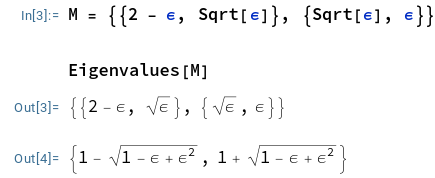
\includegraphics[scale=0.5]{MatrixEigenValues.png}
        \end{center}
        Both of these eigenvalues are positive, so the matrix is semi-positive definite.


        Now calculating the probablility of outcome $1$ gives:
        \begin{align*}
          P(1) &= \langle 1 | E_1| 1 \rangle \\
               &= \langle 1 | \frac{1}{2}\left[(2 - \epsilon)|1\rangle \langle 1| - \sqrt{\epsilon} |1\rangle \langle 0| - \sqrt{\epsilon} |0\rangle \langle 1| + \epsilon |0\rangle \langle 0|\right] | 1 \rangle\\
               &= 1 - \frac{1}{2} \epsilon
        \end{align*}
      \item
        The faulty measurement here for $\sigma_z$ is:
        \begin{align*}
          \hat \sigma_z 
                    &= (1 - \epsilon)|1\rangle \langle 1| - \sqrt{\epsilon} |1\rangle \langle 0| - \sqrt{\epsilon} |0\rangle \langle 1| + \epsilon |0\rangle \langle 0| \\
                    & \qquad - \left[(1 - \epsilon)|0\rangle \langle 0| + \sqrt{\epsilon} |1\rangle \langle 0| + \sqrt{\epsilon} |0\rangle \langle 1| + \epsilon |1\rangle \langle 1|\right]\\
                    &= (1 - 2\epsilon)|1\rangle \langle 1| - 2 \sqrt{\epsilon} |1\rangle \langle 0| - 2 \sqrt{\epsilon} |0\rangle \langle 1| - (1 - 2\epsilon) |0\rangle \langle 0|
        \end{align*}
        Now to calculate the $r_z$ component:
        \begin{align*}
          r_z &= \tr{\rho\sigma_z} \\
              &= \tr{| 0\rangle \langle 0|[(1 - 2\epsilon)|1\rangle \langle 1| - 2 \sqrt{\epsilon} |1\rangle \langle 0| - 2 \sqrt{\epsilon} |0\rangle \langle 1| - (1 - 2\epsilon) |0\rangle \langle 0|]} \\
              &= \tr{[- 2 \sqrt{\epsilon} |0\rangle \langle 1| - (1 - 2\epsilon) |0\rangle \langle 0|]} \\
              &=  - (1 - 2\epsilon) \\
              &=  - 1 + 2\epsilon 
        \end{align*}
    \end{enumerate}
  \item
    \begin{enumerate}
      \item
        Expanding $U$, we get:
        \begin{align*}
          \hat U &= e^{i \theta \hat \sigma_z \otimes \hat \sigma_z}\\
                 &= \sum_{n = 0}^\infty \frac{1}{n!}\left(i \theta \hat \sigma_z \otimes \hat \sigma_z\right)\\
                 &= \sum_{n = 0}^\infty \frac{1}{n!}
                   \left[
                      i \theta
                      \left( 
                        \begin{matrix}
                          1 & 0 & 0 & 0 \\
                          0 &-1 & 0 & 0 \\
                          0 & 0 &-1 & 0 \\
                          0 & 0 & 0 & 1
                        \end{matrix}
                      \right)
                    \right]^n\\
                  &= \sum_{n \text{ even}}^\infty \frac{1}{n!}
                   \left[
                      i \theta
                      \left( 
                        \begin{matrix}
                          1 & 0 & 0 & 0 \\
                          0 & 1 & 0 & 0 \\
                          0 & 0 & 1 & 0 \\
                          0 & 0 & 0 & 1
                        \end{matrix}
                      \right)
                    \right]^n
                  + \sum_{n \text{ odd}}^\infty \frac{1}{n!}
                   \left[
                      i \theta
                      \left( 
                        \begin{matrix}
                          1 &  0 &  0 & 0 \\
                          0 & -1 &  0 & 0 \\
                          0 &  0 & -1 & 0 \\
                          0 &  0 &  0 & 1
                        \end{matrix}
                      \right)
                    \right]^n\\
                  &= 
                   \left[
                      \left( 
                        \begin{matrix}
                          \cos \theta & 0 & 0 & 0 \\
                          0 & \cos \theta & 0 & 0 \\
                          0 & 0 & \cos \theta & 0 \\
                          0 & 0 & 0 & \cos \theta
                        \end{matrix}
                      \right)
                    \right]
                  + 
                   \left[
                      \left( 
                        \begin{matrix}
                          i\sin \theta &  0 &  0 & 0 \\
                          0 & -i\sin \theta &  0 & 0 \\
                          0 &  0 & -i\sin \theta & 0 \\
                          0 &  0 &  0 & i\sin \theta
                        \end{matrix}
                      \right)
                    \right]\\
                  &= \cos \theta I_4 + i \sin \theta \hat\sigma_z \otimes \hat \sigma_z
        \end{align*}
        And therefore, the output of the channel is:
        \begin{align*}
          \hat \rho_E' &= \tr_S(\hat U \hat \rho_S \otimes \hat \rho_E \hat U^\dagger)\\[10pt]
                       &= \tr_S((\cos \theta I_4 + i \sin \theta \hat\sigma_z \otimes \hat \sigma_z) \hat \rho_S \otimes \hat \rho_E (\cos \theta I_4 - i \sin \theta \hat\sigma_z \otimes \hat \sigma_z))\\[10pt]
                       &= \cos^2 \theta\tr_S( \hat \rho_S \otimes \hat \rho_E ) + i \tr_S(\sin \theta \hat\sigma_z \otimes \hat \sigma_z \hat \rho_S \otimes \hat \rho_E \cos \theta I_4)\\
                       & \qquad - i\tr_S(\cos \theta I_4 \hat \rho_S \otimes \hat \rho_E \sin \theta \hat\sigma_z \otimes \hat \sigma_z) + \sin^2 \theta \tr_S( \hat\sigma_z \otimes \hat \sigma_z \rho_S \otimes \hat \rho_E \hat\sigma_z \otimes \hat \sigma_z)\\[10pt]
                       &= \cos^2 \theta\tr_S( \hat \rho_S \otimes \hat \rho_E ) + i \sin \theta \cos \theta \tr_S( \hat\sigma_z \otimes \hat \sigma_z \hat \rho_S \otimes \hat \rho_E  I_4)\\
                       & \qquad - i \sin \theta \cos \theta \tr_S(I_4 \hat \rho_S \otimes \hat \rho_E \hat\sigma_z \otimes \hat \sigma_z) + \sin^2 \theta \tr_S( \hat\sigma_z \otimes \hat \sigma_z \rho_S \otimes \hat \rho_E \hat\sigma_z \otimes \hat \sigma_z)\\[10pt]
                       &= \cos^2 \theta\tr_S( \hat \rho_S \otimes \hat \rho_E ) + i \sin \theta \cos \theta \tr_S( \hat\sigma_z \otimes \hat \sigma_z \hat \rho_S \otimes \hat \rho_E)\\
                       & \qquad - i \sin \theta \cos \theta \tr_S(\hat \rho_S \otimes \hat \rho_E \hat\sigma_z \otimes \hat \sigma_z) + \sin^2 \theta \tr_S( \hat\sigma_z \otimes \hat \sigma_z \rho_S \otimes \hat \rho_E \hat\sigma_z \otimes \hat \sigma_z)\\[10pt]
                       &= \cos^2 \theta\tr_S( \hat \rho_S \otimes \hat \rho_E ) + i \sin \theta \cos \theta \tr_S( \hat\sigma_z \hat \rho_S \otimes \hat \sigma_z \hat \rho_E)\\
                       & \qquad - i \sin \theta \cos \theta \tr_S(\hat \sigma_z\hat \rho_S \otimes \hat \rho_E \hat \sigma_z) + \sin^2 \theta \tr_S(\rho_S \otimes \hat \sigma_z \rho_E  \hat \sigma_z)\\[10pt]
                       &= \cos^2 \theta\tr_S( \hat \rho_S \otimes \hat \rho_E ) + i \sin \theta \cos \theta \tr_S( \hat\sigma_z \hat \rho_S \otimes [\hat \sigma_z, \hat \rho_E])  + \sin^2 \theta \tr_S(\rho_S \otimes \hat \sigma_z \rho_E  \hat \sigma_z)
  %                     &= \tr_S(\hat U \hat \rho_S \otimes \hat \rho_E \hat U^\dagger)\\
  %                     &= \tr_S(e^{i \theta \hat\sigma_z \otimes \hat\sigma_z} \hat \rho_S \otimes \hat \rho_E e^{-i \theta \hat\sigma_z \otimes \hat\sigma_z})\\
  %                     &= \tr_S(e^{i \theta \hat\sigma_z \hat \rho_S \hat\sigma_z \otimes \hat\sigma_z \hat \rho_E \hat\sigma_z}  )\\
      \end{align*}
    \item
      The density matrix for this entangeled state is:
      \begin{align*}
        \hat \rho_{SS'} &= |\Phi^+\rangle\langle\Phi^+|\\
                        &= \frac{1}{2}\left(|0_S0_{S'}\rangle\langle 0_S0_{S'}| + |0_S0_{S'}\rangle\langle 1_S1_{S'}| + |1_S1_{S'}\rangle\langle 0_S0_{S'}| + |1_S1_{S'}\rangle\langle 1_S1_{S'}|\right)
      \end{align*}
      Therefore:
      \begin{align*}
        \hat \rho'_{ES'} &= (\Phi \otimes I) (\hat \rho_{SS'})\\
                         &= \cos^2 \theta\tr_S( \hat \rho_{SS'} \otimes \hat \rho_E ) + i \sin \theta \cos \theta \tr_S( \hat\sigma_z \hat \rho_{SS'} \otimes [\hat \sigma_z, \hat \rho_E])  + \sin^2 \theta \tr_S(\rho_{SS'} \otimes \hat \sigma_z \rho_E  \hat \sigma_z)
      \end{align*}
      Now:
      \begin{align*}
        \cos^2 \theta\tr_S( \hat \rho_{SS'} \otimes \hat \rho_E ) = \frac{1}{2}\cos^2 \theta(|0_{S'}\rangle\langle 0_{S'}| \otimes |0_E\rangle\langle 0_E| + |1_{S'}\rangle\langle 1_{S'}| \otimes |0_E\rangle\langle 0_E|)
      \end{align*}
      and for the second term:
      \begin{align*}
          & i \sin \theta \cos \theta \tr_S( \hat\sigma_z \hat \rho_{SS'} \otimes [\hat \sigma_z, \hat \rho_E]) \\
        = & i \sin \theta \cos \theta \tr_S( \hat\sigma_z \hat \rho_{SS'} \otimes [|1_E\rangle\langle1_E| - |0_E\rangle\langle0_E|, |0_E\rangle \langle 0_E|]) \\
        = & i \sin \theta \cos \theta \tr_S( \hat\sigma_z \hat \rho_{SS'} \otimes 0) \\
        = & 0
      \end{align*}
      And for the last term:
      \begin{align*}
          & \sin^2 \theta \tr_S(\rho_S \otimes \hat \sigma_z \rho_E  \hat \sigma_z)\\
        = & \sin^2 \theta \tr_S\left( \frac{1}{2}\left(|0_S0_{S'}\rangle\langle 0_S0_{S'}| + |0_S0_{S'}\rangle\langle 1_S1_{S'}| + |1_S1_{S'}\rangle\langle 0_S0_{S'}| + |1_S1_{S'}\rangle\langle 1_S1_{S'}|\right)\otimes |0_E\rangle \langle 0_E| \right)\\
        = & \frac{1}{2} \sin^2 \theta  \left(|0_{S'}\rangle\langle 0_{S'}| + |1_{S'}\rangle\langle 1_{S'}|\right)\otimes |0_E\rangle \langle 0_E|\\
      \end{align*}
      Therefore:
      \begin{align*}
        \hat \rho'_{ES'} = \frac{1}{2}\left(|0_{S'}\rangle \langle 0_{S'}| + |1_{S'}\rangle \langle 1_{S'}|\right) \otimes |0_E\rangle \langle 0_E|
      \end{align*}
      Which is a product state, and therefore separable.
    \item
      I am not sure about the answer I have here, but anyway.
      Using the spectral decomposition of $A$:
      \begin{align*}
        U &= e^{i \theta \hat A \otimes \hat B}\\
          &= e^{i \theta \sum_j c_j \hat P_j \otimes \hat B}\\
          &= e^{\sum_j \hat P_j \otimes i \theta c_j \hat B}\\
          &= \sum_j \hat P_j \otimes e^{  i\theta c_j  \hat B}
      \end{align*}
      Putting this in the channel gives:
      \begin{align*}
        \Phi(\hat \rho_S) &= \tr_S\left(\left[\sum_j \hat P_j \otimes e^{  i\theta c_j  \hat B}\right] \hat \rho_S \otimes \hat \rho_E \left[\sum_k \hat P_k \otimes e^{ -i\theta c_k  \hat B}\right]\right)\\
                          &= \sum_j \sum_k \tr_S\left(\hat P_j   \hat \rho_S \hat P_k \otimes e^{  i\theta c_j  \hat B}\hat \rho_E  e^{- i\theta c_k  \hat B}\right)\\
                          &= \sum_j \sum_k \tr_S\left( \hat P_j \hat P_k \hat \rho_S \otimes e^{  i\theta c_j  \hat B}\hat \rho_E  e^{- i\theta c_k  \hat B}\right)\\
                          &= \sum_j \tr_S\left( \hat P_j \hat \rho_S  \otimes e^{  i\theta c_j  \hat B}\hat \rho_E  e^{- i\theta c_j  \hat B}\right)\\
                          &= \sum_j \tr_S\left( \hat P_j \hat \rho_S  \otimes I\right) I \otimes e^{  i\theta c_j  \hat B}\hat \rho_E  e^{- i\theta c_j  \hat B}
      \end{align*}
      Now in the above, the set of orthogonal projectors $\{P_j\}$ form a POVM (they are a set of PVMs).
      $I \otimes e^{  i\theta c_j  \hat B}\hat \rho_E  e^{- i\theta c_j  \hat B}$ is a unitary transformation of density matrix and hence a density operator.
    \end{enumerate}
\end{enumerate}
\end{document}
